\documentclass[a4paper,12pt]{article}

\usepackage{fancyhdr}
\lhead{\footnotesize{Project CUDC Report}}
\lfoot{\footnotesize{CS 217 Fall 2015}}
\rfoot{\footnotesize{OUNAN DING 861194909}}
\pagestyle{fancy}

\usepackage{hyperref}

\usepackage{amsmath}

% For \mathds
\usepackage{dsfont}

\usepackage{tikz}

\usepackage{graphicx}

\title{Project CUDC Report}
\date{}
\author{
OUNAN DING\\
Student ID: 861194909\\
oding001@ucr.edu
}

\begin{document}

\maketitle{}

\tableofcontents{}

\section{Overview}

This report is for the final project of CS/EE-217 GPU Architecture
and Programming.
Implementations of dual contouring will be presented and analyzed.

We provide a CPU implementation written in C\texttt{++} first as our baseline,
then move on to introduce the CUDA implementations.
We will see what the bottle neck is in our CPU version,
and how we make trade off in the CUDA version to overcome that bottle neck.
A visualizer is also provided as a Blender add-on
to preview the results and check the correctness.

Finally we will provide some performance testing and detailed analysis
in the last part of this report.

\section{Design and Implementation}

\subsection{General Overview}

In this section we will provide a general overview of dual contouring.
The architecture-independent perspectives
of this algorithm will be discussed.

The primary paper used for this project is \cite{ju2002dual}.
\cite{schaefer2002dual} also provides supplemental materials
on how to construct and solve the Quadratic Error Function(QEF).

For the first step in dual contouring, given an implicit function
such as $(x^2 + y^2 - 1)^3 - x^2y^3$ in 2D, or $x^2 + y^2 + z^2 - 1$ in 3D,
we will sample the function on a uniform grid.
Here is an example in figure \ref{fig:sampling-2d-dc},
where we sample the function $x^2 + y^2 - 1.7$.
The $0$ level set of this function is plotted as a circle of radius $1.7$.
The samples which have a negative value are drawn with filled dots.

\begin{figure}[h]
\centering
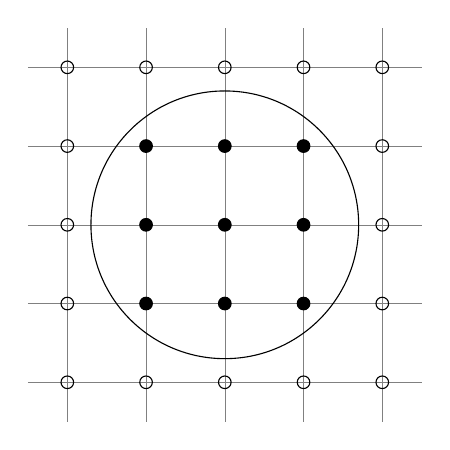
\begin{tikzpicture}

\draw[step=1, gray, very thin] (-2.5, -2.5) grid (2.5, 2.5);
\draw (0, 0) circle (1.7);

\draw (-2, -2) circle (0.08);
\draw (-1, -2) circle (0.08);
\draw (0, -2) circle (0.08);
\draw (1, -2) circle (0.08);
\draw (2, -2) circle (0.08);

\draw (-2, -1) circle (0.08);
\filldraw (-1, -1) circle (0.08);
\filldraw (0, -1) circle (0.08);
\filldraw (1, -1) circle (0.08);
\draw (2, -1) circle (0.08);

\draw (-2, 0) circle (0.08);
\filldraw (-1, 0) circle (0.08);
\filldraw (0, 0) circle (0.08);
\filldraw (1, 0) circle (0.08);
\draw (2, 0) circle (0.08);

\draw (-2, 1) circle (0.08);
\filldraw (-1, 1) circle (0.08);
\filldraw (0, 1) circle (0.08);
\filldraw (1, 1) circle (0.08);
\draw (2, 1) circle (0.08);

\draw (-2, 2) circle (0.08);
\draw (-1, 2) circle (0.08);
\draw (0, 2) circle (0.08);
\draw (1, 2) circle (0.08);
\draw (2, 2) circle (0.08);

\end{tikzpicture}
\caption{Sampling of $x^2 + y^2 - 1.7$}
\label{fig:sampling-2d-dc}
\end{figure}

Every edge which exhibits opposite signs at its ends
has a potential intersection with the $0$ level set of the function.
We highlight these edges in figure \ref{fig:intersected-edges-2d-dc}.

\begin{figure}[h]
\centering
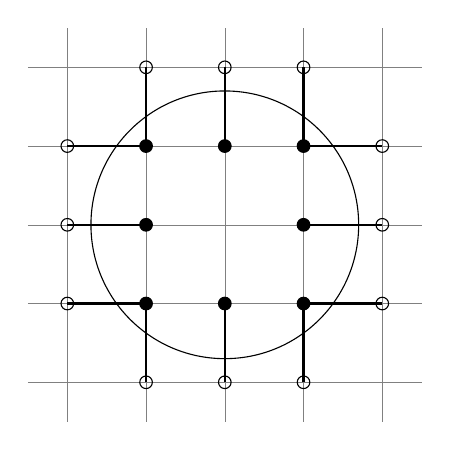
\begin{tikzpicture}
\draw[step=1, gray, very thin] (-2.5, -2.5) grid (2.5, 2.5);
\draw (0, 0) circle (1.7);

\draw (-1, -2) circle (0.08);
\draw (0, -2) circle (0.08);
\draw (1, -2) circle (0.08);

\draw (-2, -1) circle (0.08);
\filldraw (-1, -1) circle (0.08);
\filldraw (0, -1) circle (0.08);
\filldraw (1, -1) circle (0.08);
\draw (2, -1) circle (0.08);

\draw (-2, 0) circle (0.08);
\filldraw (-1, 0) circle (0.08);
\filldraw (1, 0) circle (0.08);
\draw (2, 0) circle (0.08);

\draw (-2, 1) circle (0.08);
\filldraw (-1, 1) circle (0.08);
\filldraw (0, 1) circle (0.08);
\filldraw (1, 1) circle (0.08);
\draw (2, 1) circle (0.08);

\draw (-1, 2) circle (0.08);
\draw (0, 2) circle (0.08);
\draw (1, 2) circle (0.08);

% Draw intersected edges.
\draw[thick] (-1, -2) -- (-1, -1);
\draw[thick] (0, -2) -- (0, -1);
\draw[thick] (1, -2) -- (1, -1);

\draw[thick] (-2, -1) -- (-1, -1);
\draw[thick] (1, -1) -- (2, -1);

\draw[thick] (-2, 0) -- (-1, 0);
\draw[thick] (1, 0) -- (2, 0);

\draw[thick] (-2, 1) -- (-1, 1);
\draw[thick] (-1, 1) -- (-1, 2);
\draw[thick] (0, 1) -- (0, 2);
\draw[thick] (1, 1) -- (2, 1);
\draw[thick] (1, 1) -- (1, 2);

\end{tikzpicture}
\caption{The intersected edges}
\label{fig:intersected-edges-2d-dc}
\end{figure}

The intersections of these edges can be found by a binary search.
And the gradients at the intersections
(the Hermitian data in the glossary of \cite{ju2002dual})
can be computed by finite differencing.
The result of this step is illustrated in figure \ref{fig:intersections-2d-dc}.

\begin{figure}[h]
\centering
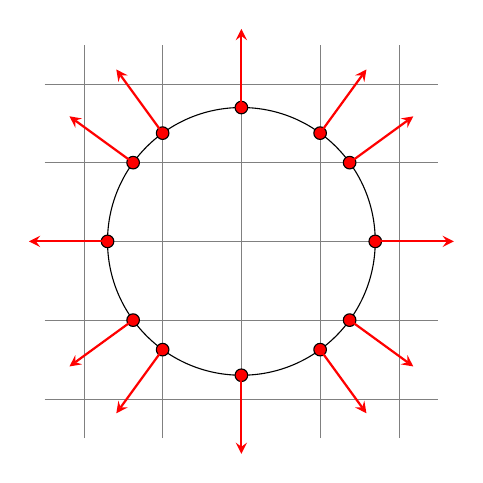
\begin{tikzpicture}
\draw[step=1, gray, very thin] (-2.5, -2.5) grid (2.5, 2.5);
\draw (0, 0) circle (1.7);

% Draw intersections.
\filldraw[fill=red] (-1, -1.3748) circle(0.08);
\filldraw[fill=red] (0, -1.7) circle(0.08);
\filldraw[fill=red] (1, -1.3748) circle(0.08);

\filldraw[fill=red] (-1.3748, -1) circle(0.08);
\filldraw[fill=red] (1.3748, -1) circle(0.08);

\filldraw[fill=red] (-1.7, 0) circle(0.08);
\filldraw[fill=red] (1.7, 0) circle(0.08);

\filldraw[fill=red] (-1.3748, 1) circle(0.08);
\filldraw[fill=red] (-1, 1.3748) circle(0.08);
\filldraw[fill=red] (0, 1.7) circle(0.08);
\filldraw[fill=red] (1, 1.3748) circle(0.08);
\filldraw[fill=red] (1.3748, 1) circle(0.08);

% Draw gradients.
\draw[->, >=stealth, thick, red] (-1, -1.3748) -- (-1.5882, -2.1835);
\draw[->, >=stealth, thick, red] (0, -1.7) -- (0, -2.7);
\draw[->, >=stealth, thick, red] (1, -1.3748) -- (1.5882, -2.1835);

\draw[->, >=stealth, thick, red] (-1.3748, -1) -- (-2.1835, -1.5882);
\draw[->, >=stealth, thick, red] (1.3748, -1) -- (2.1835, -1.5882);

\draw[->, >=stealth, thick, red] (-1.7, 0) -- (-2.7, 0);
\draw[->, >=stealth, thick, red] (1.7, 0) -- (2.7, 0);

\draw[->, >=stealth, thick, red] (-1.3748, 1) -- (-2.1835, 1.5882);
\draw[->, >=stealth, thick, red] (-1, 1.3748) -- (-1.5882, 2.1835);
\draw[->, >=stealth, thick, red] (0, 1.7) -- (0, 2.7);
\draw[->, >=stealth, thick, red] (1, 1.3748) -- (1.5882, 2.1835);
\draw[->, >=stealth, thick, red] (1.3748, 1) -- (2.1835, 1.5882);

\end{tikzpicture}
\caption{Intersections and their Hermitian data}
\label{fig:intersections-2d-dc}
\end{figure}

After the Hermitian data is ready,
the QEFs can be built.

\begin{eqnarray*}
E[x] & = & \sum_i {(n_i \cdot (x - p_i))^2}\\
& = & x^T A^T Ax - 2x^T A^T b + b^T b
\end{eqnarray*}

In 2D dual contouring,
each QEF can be represented by $7$ floating point numbers.
Since $A^T A$ is a $2\times 2$ symmetrical matrix, it requires $3$ floats.
The $A^T b$ is a $2\times 1$ column vector, so it requires $2$ floats.
We also store $2$ floats for the mass point,
which is a $2\times 1$ column vector and will be used in mass point projection
(see \cite{schaefer2002dual} for details about mass point projection).

We solve the QEF by computing the pseudo-inverse
as suggested in \cite{ju2002dual}.
And compute a $2\times2$ SVD for the pseudo-inverse.
This method is described in \cite{blinn2003jim}.

After solving all of the QEFs, we get all vertices of the result mesh.
We can build the topology by connecting vertices from
adjacent grid cells.

Figure \ref{fig:2d-dc-example} illustrates dual contouring results
for a heart, a squircle($x^4 + y^4 - 1$),
and the subtraction of them.

\begin{figure}[h]
\centering
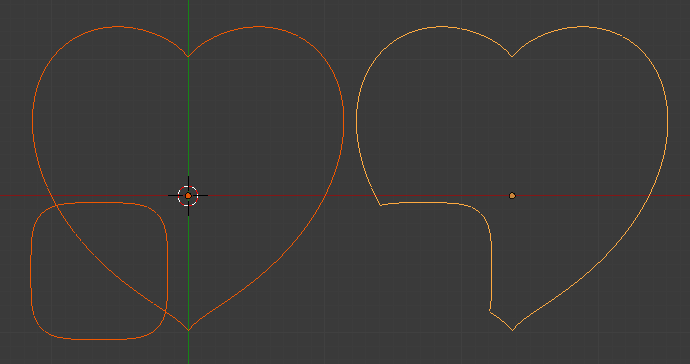
\includegraphics[width=0.9 \textwidth]{heart-squircle-subtraction.png}
\caption{2D dual contouring example}
\label{fig:2d-dc-example}
\end{figure}

\subsection{The CPU Version}

\subsection{The CUDA Version}

\section{Analysis}

\section{Conclusion}

\newpage
\addcontentsline{toc}{section}{References}
\bibliography{papers}
\bibliographystyle{alpha}

\end{document}
